
\documentclass[10pt,a4paper]{article}
    \usepackage[utf8]{inputenc}
    \usepackage{xcolor}
    % \usepackage[utf8x]{inputenc} % para poder usar tildes en archivos UTF-8
    \usepackage[spanish,es-tabla]{babel}
    \usepackage{verbatim}
    \usepackage{clrscode3e}
    \usepackage{amssymb}
    \usepackage{graphicx}
    \usepackage{float}
    \usepackage{pdfpages}
% \documentclass[10pt,a4paper]{article}
% \usepackage[utf8x]{inputenc} % para poder usar tildes en archivos UTF-8
% \usepackage[spanish,es-tabla]{babel}
% \usepackage{verbatim}
% \usepackage{amsmath}
% \usepackage{clrscode3e}
% \usepackage{amssymb}
% \usepackage{graphicx}
% \usepackage{float}
% \usepackage{pdfpages}

%\usepackage{bibtex}

%\usepackage{a4wide} % márgenes un poco más anchos que lo usual

\usepackage{caratula} % Se puede descargar en ~> https://github.com/bcardiff/dc-tex
\usepackage[breaklinks=true]{hyperref}


\begin{document} % Todo lo que escribamos a partir de aca va a aparecer en el documento.

%fran
%\sloppy

% Completar los datos de la caratula
\titulo{Trabajo Práctico 1 - Eligiendo justito} 
\fecha{\today}
\materia{Algoritmos y Estructuras Datos III}
\grupo{Grupo "Kubrak"}

% Completar los integrantes del grupo:)
\integrante{Cristian Kubrak}{456/15}{Kubrakcristian@gmail.com}


\maketitle
\par \textbf{Abstract:} El objetivo de este trabajo es resolver el problema de la suma de
subconjuntos mediante 3 diferentes t\'ecnicas: Fuerza Bruta, Backtracking y 
Programaci\'on din\'amica para luego analizar cu\'al de ellas resulta mejor aplicar seg\'un el contexto.

\par  \textbf{Palabras clave:} subset sum - brute force - Backtracking - Programaci\'on din\'amica
% Aca comienzan a escribir su informe
\tableofcontents


% \newpage

\section{Introducción}
\par Dado un conjunto $S = \{v_1,v_2,...,v_n\}$, y un valor objetivo $V$, se busca decidir si existe un subconjunto
de items de $S$ que sumen exactactamente el valor objetivo $V$. En caso de existir dicho conjunto, se obtener la
m\'inima cardinalidad entre los subconjuntos que sumen $V$.

\par Para resolver este problema, se utilizaron tres t\'ecnicas diferentes: \emph{Fuerza Bruta}, \emph{BackTracking}
y \emph{Programaci\'on din\'amica}.

\subsubsection{Fuerza Bruta}
\par Para el caso de la fuerza bruta, se busca armar todos los posibles subconjuntos del conjunto $S$ para luego realizar
la suma y verificar si el n\'umero obtenido es $V$.

\subsubsection{BackTracking}
\par El BackTracking es un m\'etodo de fuerza bruta inteligente: en el peor caso se comporta como un m\'etodo de fuerza
bruta, pero no se investigan las posibilidades que por \emph{optimalidad } o \emph{factibilidad} se descartan.
Para descartar por \emph{optimalidad}, una vez hallada una soluci\'on se guarda el cardinal. A la hora de analizar nuevas
posibles soluciones, si el el cardinal del nuevo subconjunto excede el actual m\'inimo, es descartado. \par
Por otro lado, para descartar por \emph{factibilidad} a la hora de armar un subconjunto se lo arma elemento por elemento
y en caso de ya superar el valor $V$, se dejan de agregar elementos (ya que todos son no negativos).


\subsubsection{Programaci\'on din\'amica}
\par Para este enfoque, se plantea el problema a resolver como un problema recursivo a partir de subproblemas.
Al haber varios subproblemas superpuestos, se guarda su soluci\'on en un diccionario de r\'apido acceso. Al tener las 
soluciones al subproblema almacenadas, no se realiza m\'as de una vez la misma operaci\'on.

\subsection{Ejemplos del problema}
\subsubsection{Caso A}
Sea un conjunto $S = \{ 4, 10,3,1,1\}$ y $V=5$. Los posibles subconjuntos que suman 5 son: $\{4,1 \}$ y $\{3,1,1\}$
los cuales tienen cardinal 2 y 3 respectivamente. Dado que el inter\'es de este problema es encontrar la 
m\'inima cardinal para la cual existe un subconjunto tal que la suma de sus elementos es exactactamente $V$, la 
soluci\'on para este caso es $2$.
\subsubsection{Caso B}
Sea el conjunto $S = \{ 5, 7 ,3,2\}$ y $V=6$. No extiste ning\'un subconjunto tal que la suma de los elementos
sea exactactamente $6$, raz\'on por la soluci\'on a este problema es $-1$
\newpage

\section{Desarrollo}
\subsection{Fuerza Bruta}
Como primera opci\'on para resolver el problema se encuentra el algor\'itmo de Fuerza Bruta que, tal como el nombre
da a suponer, es una forma poco inteligente de buscar una soluci\'on ya que implica recorrer todo el \'arbol de 
soluciones:

\begin{codebox}
    \Procname{\proc{ResolverFuerzaBruta}(int V, int[] S, int i, int n) \textcolor{red}{O($2^n$)}}
    \li \If $i == -1$ \textcolor{red}{O($1$)}
        \Then
    \li        \If $V == 0$ : \textcolor{red}{O($1$)}
                \Then
    \li             \Return $0$ \textcolor{red}{O($1$)}
    \li         \Else: 
    \li                 \Return $n+1$\footnote{Si el algor\'itmo devulve un n\'umero mayor que $n$ significa que no existe soluci\'on} \textcolor{red}{O($1$)}
                \End
                \End

    \li \Return min(ResolverFuerzaBruta($V$,$S$,$i-1$,$n$), \\
   $\quad\quad\quad\quad\quad$ $1 +$ResolverFuerzaBruta($V-S[i]$,$S$,$i-1$,$n$)) \textcolor{red}{O($2^n$)}

    \end{codebox}


\begin{figure}[H] 
\centering
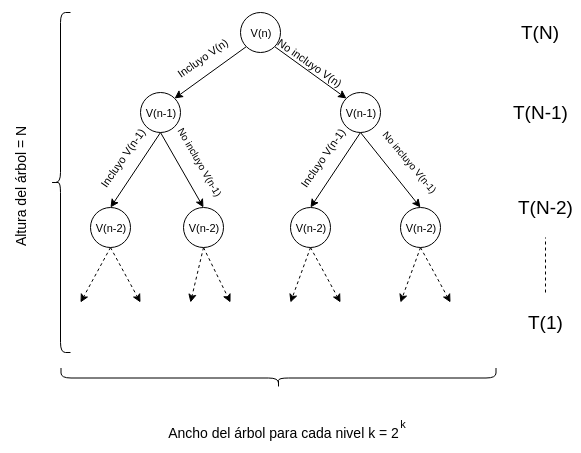
\includegraphics[width=.8\textwidth]{img/arbolRecurrencia.png}
\caption{\'Arbol de recurrencia}
\label{fig:arbolRecurrencia}
\end{figure}

Como la altura del \'arbol es de $n$ (el tama\~no del conjunto $S$) y el $\forall k, 1\leq k \leq n$ el ancho del
\'arbol para el nivel $k$ es de $2^k$, para recorrer todo el \'arbol se requieren:
\begin{equation}
    \sum_{i=0}^{n-1} 2^i*O(1) = \frac{2^{n}}{2-1} = 2^{n} \in O(2^n)
\end{equation}
Como se requieren $O(2^n)$ operaciones para investigar todas las soluciones y efectivamente se las investiga todas,
la complejidad del Fuerza Bruta es exactamente $O(2^n)$.

\subsection{Back Tracking}

\begin{codebox}
    \Procname{\proc{ResolverBackTracking}(int V, int[] S, int i, int n, int minParcial, int cardinalParcial) \textcolor{red}{O($2^n$)}} 
    % \li \If $i == -1$ \textcolor{red}{O($n*2^n$)}
    \li \If $cardinalParcial$ $>$ $minParcial$: \textcolor{red}{O($1$)}
        \Then
    \li        \Return $n+1$ \footnote{\label{bktrk}Si el algor\'itmo devulve un n\'umero mayor que $n$ significa que no existe soluci\'on} \End\textcolor{red}{O($1$)}
    \li \If $V == 0$: \textcolor{red}{O($1$)}
         \Then
    \li         $minParcial = cardinalParcial$ \textcolor{red}{O($1$)}
    \li         \Return $0$ \textcolor{red}{O($1$)}
    \End
    \li \If $i == -1$ \textcolor{red}{O($1$)}
        \Then
    \li                 \Return $n+1$ \textsuperscript{\ref{bktrk}} \textcolor{red}{O($1$)}
                \End
    \li \If $S[i]$ $>$ $V$: \textcolor{red}{O($1$)}
        \Then 
    \li         \Return  ResolverBackTracking($V$,$S$,$i-1$,$n$,$minParcial$,$cardinalParcial$)\textcolor{red}{O($2^n$)}
    \li    \Else:
    \li          \Return min(ResolverBackTracking($V$,$S$,$i-1$,$n$,$minParcial$,$cardinalParcial$),\textcolor{red}{O($2^n$)}
                            \\ $\qquad\qquad$$\qquad\quad\,\,$ $1+$ ResolverBackTracking($V-S[i]$,$S$,$i$,$n$,$minParcial$,$cardinalParcial+1$))



    \end{codebox}

\par Resulta f\'acil ver que la soluci\'on de Back Tracking es un caso especial del algor\'itmo de Fuerza Bruta,
salvo que gracias a las podas de \textit{optimalidad} y \textit{factibilidad} se evita investigar ciertas partes del
\'arbol de soluci\'on. A\'un as\'i, en el peor caso (por ejemplo un arreglo en el cual la suma de sus elementos no llega
a $V$) se termina comportando como Fuerza Bruta. Luego su complejidad resulta $O(2^n)$

\subsubsection{Poda por factibilidad}
\par La poda por \textit{factibilidad} se realiza en en la l\'inea 9 del pseudoc\'odigo. La misma consiste en
evaluar si el $S[i]$ es mayor estricto que el $V$. De as\'i serlo se excluye tal elemento en la soluci\'on ya que obviamente
har\'a que la suma de cualquier subconjunto que lo incluya exceder\'a el valor de $V$.


\subsubsection{Poda por optimalidad}
\par La poda por optimalidad se realiza en la l\'inea 1 del pseudoc\'odigo aunque las operaciones gracias a las
cuales funciona esta poda se realizan en las l\'ineas 4 y 12. En la primer l\'inea se evalua si el $cardinalParcial$
(el cardinal que lleva el subconjunto actual) es mayor estricto a $minParcial$ (el m\'inimo cardinal para el que
se encontr\'o un subconjunto cuya suma es exactamente $V$); de as\'i serlo, no tiene relevancia seguir evaluando
esa rama del \'arbol de soluciones ya que en caso de encontrar un subconjunto cuya suma sea $V$, su cardinal no ser\'a
el m\'inimo.
\par En la l\'inea 12, si se encontr\'o un subconjunto cuya suma sea $V$ (n\'otese que el $cardinalParcial$ debe
ser menor o igual al $minParcial$ gracias a la condici\'on en la l\'inea 1), $cardinalParcial$ pasa a ser el nuevo
$minParcial$ y se llega al caso base, por lo que se devuelve 0.
\par En la l\'inea 11 se busca el m\'inimo evaluan dos casos: incluir o no el elemento $S[i]$. N\'otese que en caso
de incluirlo el $cardinalParcial$ aumenta en 1.

\subsection{Programaci\'on Din\'amica}
\subsubsection{Correctitud}
Caracterizaci\'on de una solución \textbf{óptima} S para el problema original:
\par - Si $n \not\in$ $S$, entonces la mejor solución es $S =S_1$, siendo $S_1$ solución
óptima para \{$v_1 , v_2 , v_3 ,..., v_{n}$\} llegando al valor objetivo $V$
\par - Si $n \in S$, entonces la mejor solución es $S = \{n\} \cup S_2$, siendo $S_2$
solución óptima para \{$v_1 , v_2 , v_3 ,..., v_{n}$\} llegando al valor objetivo $V - v_n$
\par Por lo tanto, como esas son las únicas dos posibilidades, $S$ deberá ser la que use menos elementos entre 
$S_1$ y $\{n\} \cup S_2$
\par Usando esta caracterización, puedo elaborar una recursión
que calcule la cantidad óptima de elementos necesarios:
\begin{equation*}
  f(i,V)=\begin{cases}
    $\qquad\qquad$0 & \text{si $i=0$, $V=0$}.\\
    $\qquad\qquad$\infty & \text{si $i=0$, $V\neq 0$}.\\
    $\qquad\;\;\;$f($i$ $-$ $1$,$V$) & \text{si $i> 0$, $v_i > 0$}.\\
    min (f($i$ $-$ $1$,$V$),f($i$ $-$ $1$,$V$)) & \text{si $i> 0$, $v_i > 0$}.\\
  \end{cases}
\end{equation*}
\subsubsection{Principio de optimalidad}
\par Se puede ver que para este problema se puede aplicar el principio de optimalidad: una secuencia \'optima de
decisiones esta formada por subsecuencias que a su vez son \'opitmas.
Sea un conjunto $S$ donde $|S|=n$, $S_1\subset S$ el subconjunto \'optimo 
para los elementos $v_1, ... , v_i$  y valor objetivo
$V_1$ y $S_2\subset S$ el subconjunto \'optimo para los elementos $v_1, ..., v_{i-1}$ para formar $V_2$.
Supongo que puedo formar un conjunto $S' = S_2\cup {v_i}$, luego $|S'| = |S_2| + 1$ y $V'= V_2 + v_i'$.
\par Si $S'$ fuese \'optimo luego $V'\neq V_1$ entonces $V'\neq V_1$. Pero si $S'\neq S=S_1$ 
y $S'$ es \'optimo lo cual es
absurdo ya que $S_1$ es \'optimo tomando $v_1,...,v_i$ entonces $S_1=S_2$ y $V_1 = V_2$.
\par Entonces, se cumple es principio de optimalidad.

\begin{codebox}
    \Procname{\proc{ResolverDinamica}(int V, int[] S, int i, int n, matriz resultados) \textcolor{red}{O($n*V$)}}
    \li \If $V == 0$: \textcolor{red}{O($1$)}
        \Then
         \li       \Return $0$ \textcolor{red}{O($1$)}
                \End
    \li \If $i == -1$ or $V<0$  \textcolor{red}{O($1$)}
        \Then
    \li                 \Return $n+1$\footnote{\label{bktrk}Si el algor\'itmo devulve un n\'umero mayor que $n$ significa que no existe soluci\'on} \textcolor{red}{O($1$)}
                \End
    \li \If $noEstaDefinido(resultados[i][V]$):  \textcolor{red}{O($1$)}
        \Then 
    \li          resultados[i][vDeseado] = min(ResolverDinamica($V$,$S$,$i-1$,$n$,$resultados$,
                            \\ $\qquad\qquad\qquad\qquad\qquad\qquad$$\qquad\quad\,\,$ $1+$ResolverDinamica($V-S[i]$,$S$,$i-1$,$n$,$resultados$)) \textcolor{red}{O($n*V$)}
                            \End
    \li \Return resultados[i][vDeseado]  \textcolor{red}{O($1$)}
    \end{codebox}
% \par Para el caso de Programaci\'on Din\'amica, la complejidad resulta $O(n*V)$ ya que cada soluci\'on parcial 
% se calcula hasta una sola vez para luego almacerlo en una matriz de $n$ filas y $V$ columnas. Si la soluci\'on al
% problema de para un valor objetivo $V'$ y un una cantidad de elementos $i$, 
\par El algor\'itmo de Programaci\'on Din\'amica busca obtener una ventaja a partir de encarar al problema como
subproblemas recursivos pero, teniendo en cuenta que hay subproblemas que se calculan m\'as de una vez, se 
almacenan las subsoluciones  en una matriz de $n$ filas y $V$ columnas la cual es inicializada con basura (alg\'un n\'umero negativo)
en todos sus posiciones a modo de identificar las soluciones calculadas.
 El objetivo de guardar las soluciones es poder acceder a ellas
r\'apidamente. Es por esto que decidi\'i utilizar para almacenar las soluciones una matriz formada por un vector de 
vectores, permiti\'endome acceder en $O(1)$ a las soluciones ya calculadas.
\par Para un $V$ fijo, existen a lo sumo $n$ subproblemas para analizar. Luego, como $V$ o bien sigue igual o se le resta $S[i]$ ($S[i]\geq 0$ $\forall 1\leq i \leq n$)
existen a lo sumo $V$ valores objetivos que se investigan. Esto resulta en que se calculen $n*V$ soluciones, y dado que el resto de las operaciones de 
la funci\'on son constantes, la complejidad final resulta $O(n*V)$.
% \par La cantidad de posibles subproblemas es $n*V$: en cada llamada o bien se reduce $i$ (el indicador
% de cu\'al elemento de $S$ estoy analizando, $i<n$) o tambi\'en el valor $V$. Es por esto que para un $V$ existen a lo sumo $n$ subproblemas
% posibles.
\newpage

\section{Ap\'endice}
\begin{figure}[H] 
    \centering
        \centering
        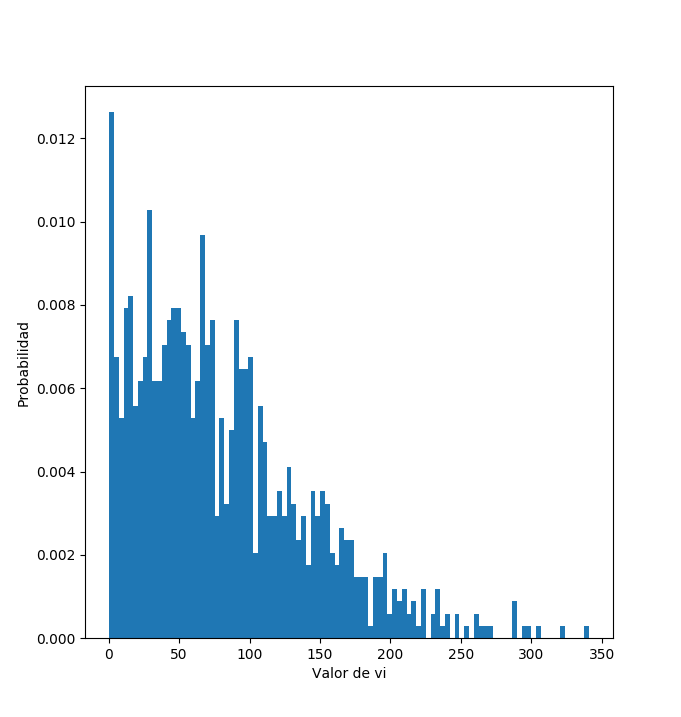
\includegraphics[width=0.7\textwidth]{img/distribucion.png} % first figure itself
        \caption{Ejemplo de la distribuci\'on ``aleatoria'' utlizada en la experimentaci\'on para 
        $n = 1000$ y $vDeseado = 500$}
        \label{fig:tiempoBackDinamicavChico} 
\end{figure}
\newpage



\end{document}

